\section{Theoretical Analysis}
\label{sec:analysis}

<<<<<<< HEAD
\paragraph{} The values used in both analysis are the following:

$R_1$ = 1.00781211614 $k\Omega$
$R_2$ = 2.00311223204 $k\Omega$
$R_3$ = 3.04503555589 $k\Omega$
$R_4$ = 4.17896607062 $k\Omega$
$R_5$ = 3.10615699135 $k\Omega$
$R_6$ = 2.06090154363 $k\Omega$
$R_7$ = 1.00634569025 $k\Omega$
$V_s$ = 5.04864033546 V
$C$ = 1.02502620056 mA
$K_b$ = 7.05958243797 mS
$K_c$ = 8.03913881798 $m\Omega$

\subsection{Analysis for t<0}

\paragraph{} For t<0 we can see that we are working in the steady state, given that in that time interval $v_S$ = $V_S$. In a DC circuit, the capacitor charges up to it's full capacity, blocking the flow of electricity. Taking 
this into account we can replace the capacitor with an open circuit. With this information, and knowing that the the tension in $V_4$, since it is connected to ground, we can obtain the following equations.

\begin{equation}
\begin{bmatrix}
	-1	&	0	&	0	&	0	&	0	&	0	&	0 \\
	G_1	&	-G_1 - G_2 - G_3	&	G_2	&	G_3	&	0	&	0	&	0 \\
	0	&	-K_b - G_2	&	G_2	&	K_b	&	0	&	0	&	0 \\
	G_1	&	-G_1	&	0	&	-G_4	&	0	&	-G_6	&	0 \\
	0	&	0	&	0	&	0	&	0	&	G_6 + G_7	&	-G_7 \\
	0	&	0	&	0	&	0	&	-1	&	0	&	1
\end{bmatrix}
\times
\begin{bmatrix}
	V_1 \\
	V_2 \\
	V_3 \\
	V_5 \\
	V_6 \\
	V_7 \\
	V_8
\end{bmatrix}
=
\begin{bmatrix}
	0 \\
	0 \\
	0 \\
	0 \\
	0 \\
	0 \\
	V_x
	\label{m:1}
\end{bmatrix}
\end{equation}

After solving them with the Octave sofware, we obtained the following results:

\begin{table}[hbt!]
  \centering
  \begin{tabular}{|l|r|}
    \hline    
    {\bf Name} & {\bf Value [mA]} \\ \hline
    $I_{a}$ & -0.186554\\ \hline
$I_{b}$ & -0.195655\\ \hline
$I_{c}$ & 0.983196\\ \hline
$I_{d}$ & 1.025026\\ \hline

  \end{tabular}
  \caption{Mesh currents expressed in mA}
  \label{tab:op}
\end{table}





=======
>>>>>>> bcb9d6dfe0f08d333c8cf6336dee07f037fc5080
\paragraph{} In this section, the circuit shown in Figure 1 is analysed using the Mesh and Node Methods, after which both results are compared.
Those methods are based upon the Kirchoff Laws, and the behaviour of the elements of the circuit, which are detailed bellow.

\paragraph{} Kirchoff Laws

\paragraph{} The analysis of this circuit is based on the Kirchoff's Circuit Laws, more specifically, the Kirchoff's Current and Voltage laws (KCL and KVL). The first law states that for a given node, the sum of the electrical currents flowing out of the node is equal to the sum of currents flowing into that node. 
It can be translated into the following equation:

\begin{equation}
	\sum_{k = 1}^n I_k = 0.
	\label{eq:kcl}
\end{equation}

The second law states that the sum of all the voltages in mesh must be zero, and can be translated into the following equation:

\begin{equation}
	\sum_{k = 1}^n V_k = 0.
	\label{eq:kvl}
\end{equation}

\paragraph{}Resistor

\paragraph{}A resistor is an electrical component that poses resistance (as the name implies) to current flow, reducing it. The functioning of a resistor can be described
 by the following equation:

\begin{equation}
	V = R * I
	\label{eq:kvl}
\end{equation}

Voltage Source

\begin{itemize}
	\item Imposes a voltage V regardless of current I
	\item Zero internal resistance
\end{itemize}

Current Source

\begin{itemize}
	\item Imposes a current I regardless of voltage V
	\item Infinite internal resistance
\end{itemize}

For the simulation and analysis we will use the following values with the numerical values given:

$R_1$ = 1.00781211614 $k\Omega$
$R_2$ = 2.00311223204 $k\Omega$
$R_3$ = 3.04503555589 $k\Omega$
$R_4$ = 4.17896607062 $k\Omega$
$R_5$ = 3.10615699135 $k\Omega$
$R_6$ = 2.06090154363 $k\Omega$
$R_7$ = 1.00634569025 $k\Omega$
$V_a$ = 5.04864033546 V
$I_d$ = 1.02502620056 mA
$K_b$ = 7.05958243797 mS
$K_c$ = 8.03913881798 $m\Omega$

In the simulation we used the following simplified circuit, which is equivalent of the one given:

\begin{figure}[h] \centering
	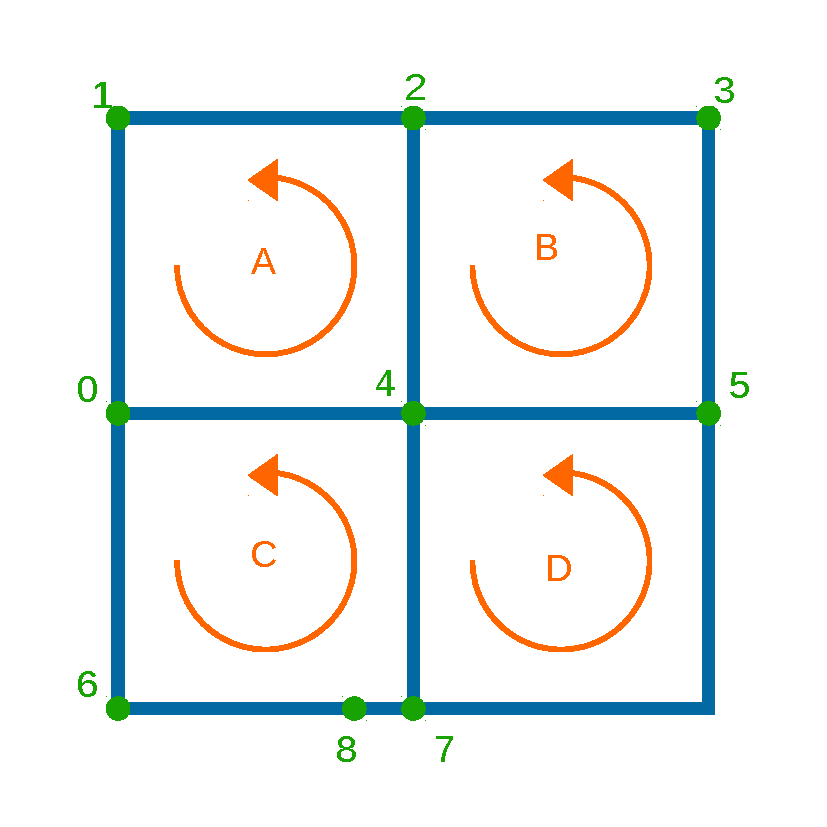
\includegraphics[width=0.4\linewidth]{sim.pdf}
	\caption{In this image you can see the number of each node as used for the simulation as well as the direction used for each mesh.}
	\label{fig:sim}
\end{figure}

\subsection{Mesh Method Analysis}

\paragraph{} After the aplication of the Mesh Method to the circuit, we obtainded the following equations:

\begin{equation}
	I_D = I_d
	\label{eq:1}
\end{equation}

\begin{equation}
	(R_1 + R_3 + R_4) I_A -R_3 I_B - R_4 I_C = - V_A
	\label{eq:1}
\end{equation}

\begin{equation}
	(R_4 + R_6 + R_7 - K_C) I_C - R_4 I_A = 0
	\label{eq:2}
\end{equation}

\begin{equation}
	(R_3 K_B - 1) I_B - R_3 K_B I_A = 0
	\label{eq:3}
\end{equation}

From which we can obtain the following matrix equation:

\begin{equation}
\begin{bmatrix}
	0 & 0 & 0 & 1 \\
	R_1 + R_3 + R_4 &  -R_3 & - R_4 & 0 \\
	-R_4 & 0 & R_4 + R_6 + R_7 - K_C & 0 \\
	-R_3 * K_B & R_3 * K_B - 1 & 0 & 0
\end{bmatrix}
\times
\begin{bmatrix}
	I_A \\
	I_B \\
	I_C \\
	I_D
\end{bmatrix}
=
\begin{bmatrix}
	I_d \\
	-V_A \\
	0 \\
	0
	\label{m:1}
\end{bmatrix}
\end{equation}


Finally, solving the problem with Octave we obtain:

\begin{table}[hbt!]
  \centering
  \begin{tabular}{|l|r|}
    \hline    
    {\bf Name} & {\bf Value [mA]} \\ \hline
    $I_{a}$ & -0.186554\\ \hline
$I_{b}$ & -0.195655\\ \hline
$I_{c}$ & 0.983196\\ \hline
$I_{d}$ & 1.025026\\ \hline

  \end{tabular}
  \caption{Mesh currents expressed in mA}
  \label{tab:op}
\end{table}

\subsection{Nodal Method Analysis}

\paragraph{} After the aplication of the Nodal Method to the circuit, we obtainded the following matrix, which in turn was obtained from the equivalent set of equations.

\begin{equation}
\begin{bmatrix}
	1 & 0 & 0 & 0 & 0 & 0 & 0 \\
	-G_1 & (G_1 + G_2+G_3) & -G_2 & -G_3 & 0 & 0 & 0 \\
	0 & (G_1 + K_B) & -G_2 & -K_B & 0 & 0 & 0 \\
	0 & K_B & 0 & (-G_5 - K_B) & G_5 & 0 & 0 \\
	0 & 0 & 0 & 0 & 0 & (G_6 + G_7) & -G_7 \\
	0 & -G_3 & 0 & (G_3 + G_4 + G_5) & -G_5 & -G_7 & G_7 \\
	0 & 0 & 0 & 1 & 0 & (K_C * G_6) & -1
\end{bmatrix}
\times
\begin{bmatrix}
	V_1 \\
	V_2 \\
	V_3 \\
	V_4 \\
	V_5 \\
	V_6 \\
	V_7
\end{bmatrix}
=
\begin{bmatrix}
	V_A \\
	0 \\
	0 \\
	I_D \\
	0 \\
	-I_D \\
	0
	\label{m:2}
\end{bmatrix}
\end{equation}

Once again, solving the matrix equation with Octave we obtain:

\begin{table}[th!]
  \centering
  \begin{tabular}{|l|r|}
    \hline    
    {\bf Name} & {\bf Value [V]} \\ \hline
    @$V_{0}$ & 0.000000\\ \hline
@$V_{1}$ & 5.048640\\ \hline
@$V_{2}$ & 4.860629\\ \hline
@$V_{3}$ & 4.468710\\ \hline
@$V_{4}$ & 4.888344\\ \hline
@$V_{5}$ & 8.679973\\ \hline
@$V_{6}$ & -2.026270\\ \hline
@$V_{7}$ & -3.015705\\ \hline

  \end{tabular}
  \caption{Node voltages expressed in V}
  \label{tab:op}
\end{table}

